\section{Prosthesis Walking Control}\label{sec:back_walking_control}

\subsection{Time Based Control}
The earliest proposed robotic prosthesis control strategy, termed \emph{echo
control}, records the kinematics of the sound-side as a function of time leg on
each step and then executes an identical trajectory on the prosthesis side on
the following step \citep{grimes1977feasibility,grimes1979active}. Such a
control strategy has a number of drawbacks. First, the control strategy requires
measurement of the sound-side leg, thus burdening the amputee with additional
sensors that need to be donned and doffed daily. Second, the control is unable
to take an odd number of steps, and all steps must be initiated with the sound
leg. Third, the control is primarily, kinematic as measuring torques of the
sound side leg to use as a feedforward control on the prosthesis is infeasible.
Consequently, it may require high-gain feedback, which may cause discomfort and
gait instability due to a lack of compliance to the environment.  

Another form of time-based control, which we will use later in this thesis, is
the minimum jerk trajectory swing control presented in \citet{lenzi2014speed}.
This swing control strategy calculates at toeoff three minimum jerk
trajectories, parameterized by $5^\tn{th}$ order polynomials, which dictate the
movement of the knee and ankle joints. For the knee joint, two trajectories are
computed, one that starts at the position, velocity, and acceleration of the
knee at toeoff and goes to a peak flexion angle with zero velocity, and one that
starts at the peak flexion state and goes to a final state of zero angle,
velocity and acceleration. The peak angle is tuned to ensure adequate foot
clearance while the acceleration at the peak angle is based on able-bodied data.
For the ankle, one minimum jerk trajectory is used that starts at the position
and velocity at toeoff and proceeds to a final position, velocity, and
acceleration of zero. The durations of the trajectories are based on fixed
percentages of the stance duration thereby automatically adapting swing phase to
different gait speeds. Unlike the previously described echo control, this
control strategy takes advantage of the simple double-pendulum dynamics during
swing to derive a strong feedforward term that allows the use of small,
compliant feedback gains.

\subsection{Finite State Impedance Control}
\begin{marginfigure}
    \centering
    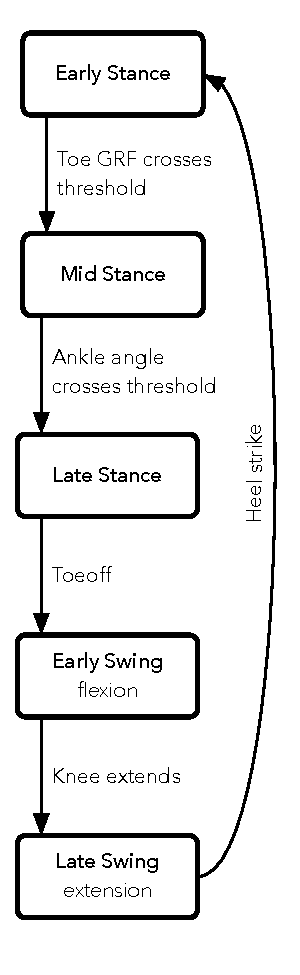
\includegraphics[width=\linewidth]{impedance_control_state_flow}
    \caption{Finite state machine used for the impedance control scheme proposed
    in \citet{sup2009preliminary}. In each state the control employs linear
    impedance functions that determine the behavior of the ankle and knee joints
    of an active transfemoral
    prosthesis.}\label{fig:impedance_control_state_flow}
\end{marginfigure}
To alleviate issues with the time-based echo control, researchers later proposed
\emph{finite state impedance control}, which has become the most widely used
control for robotic legged prostheses. In this strategy, the gait cycle is split
into a sequence of discrete states or phases. During walking, a state machine
switches between the phases based on sensor data meeting certain conditions,
usually in the form of thresholds on joint angles, joint velocities, or ground
reaction forces. Within each phase, the controller specifies an impedance
relationship between the output torque at each joint and the angle and angular
velocity of that joint.

For example, \citet{sup2009preliminary}, proposes a specific instantiation of
this control paradigm in which the gait cycle is segmented into three stance
states and two swing states as shown in \cref{fig:impedance_control_state_flow}.
In each state, the impedance of a joint is governed by
\begin{align}
    \tau = -k (\theta - \theta_{0}) - b \dot \theta,\label{eq:impedance_func}
\end{align}
where $\tau$ is the desired torque of a joint, $k$ is a stiffness parameter
$\theta_{0}$ is the joint angle offset, $b$ is a damping parameter and $\dot
\theta$ is the joint velocity. If the stiffness, damping, and offset parameters
for each joint are tuned appropriately, this control scheme can be made to suit
sloped walking \citep{sup2011upslope} and speed variations
\citep{shultz2016variable} including running \citep{shultz2015running}. There
have also been a number of variations on this general control scheme including
those with nonlinear impedance functions at the ankle
\citep{sup2007design,shultz2014walking} and some using high-gain position
control for the late stance push off phase of gait \citep{lawson2014robotic}.
\citet{lenzi2014speed} presents a similar strategy named \emph{quasi-stiffness
control} that substitutes the parameterized impedance functions given by
\cref{eq:impedance_func} with lookup tables that provide the torque vs angle
relationship at different gait speeds. 

A potential drawback of the impedance control paradigm may be its sensitivity to
the rules that govern transitions between phases. A premature transition or
delayed transition may cause inappropriate joint torques leading to gait
instabilities and falls. For this reason, prior works have experimented with a
wide variety of transition rules based on joint angles, velocities, and ground
reaction forces measured by the prosthesis. Alternatively, If one is willing to
instrument the sound-side leg, then \citet{liu2014improving} provides a method
to improve transition rules by using online learning and gait events of the
sound-side leg. In this thesis, however, we focus on control strategies that do
not require extra instrumentation of the body. Therefore, in later chapters we
will explore, through simulations (\cref{sec:control_sim}) and through
experiments with our robotic prosthesis
(\cref{sec:nm_vs_imp,sec:phase_estimation}), the potential consequences of
mistimed phase transitions in a finite state impedance control scheme that does
not use external sensing.

\subsection{Continuous Phase Control}
Another approach to walking control in active prostheses is to estimate a
continuous notion of phase. This may avoid the gait instabilities that may be
caused by joint torques changing discontinuously in finite state impedance
control. Recently, \citet{gregg2014virtual} have proposed
methods similar to the centralized virtual constraint control discussed in
\cref{sec:back_centralized_control}, in which the natural progression of a phase
variable determines the rate at which the control follows preplanned
trajectories. \citet{gregg2014virtual} chooses to follow the ankle-foot and
knee-ankle-foot rollover shapes, which are defined as the location of the center
of pressure with respect to coordinate systems attached to the shank and the
ankle-hip line respectively. The center-of-pressure naturally becomes the phase
variable for these trajectories. The observation that the roll-over shapes are
invariant across walking speed, shoe geometry, and amputee weight motivates this
choice. In this strategy, a model-based feedback linearization controller
enforces adherence to these desired trajectories as the center of pressure
progress through its natural dynamics. This formulation provides both the
feed-forward torque command and a disturbance response command that provides
exponential converge to the desired rollover shapes. 

As we noted earlier for centralized robotic control approaches, a downside of
these two trajectory following controllers is their reliance on accurate
dynamics models to compute feed-forward torques. To overcome this issue,
\citet{zhao2016first} propose a model-independent virtual constraint control. In
this scheme, quasi-stiffness control provides a feed-forward torque signal that
reduces the dependence on the model. A quadratic program then computes the
minimum required extra effort to ensure convergence to a preplanned trajectory
that is parameterized with respect to hip angle.

\begin{enumerate}
    \item Phase Variable
        \begin{enumerate}
            \item using COP
            \item using hip angle/integral
            \item splitting up into phases again
        \end{enumerate}
    \item Aaron Ames - Nonlinear control 
    \item CLME
    \item Neuromuscular Ankle
\end{enumerate}
